\section{Nico Ekklesia Sembiring}
\subsection{Apa itu fungsi library matplotlib?}
Library Matplotlib berfungsi untuk membuat visualisasi yang kuat dalam menjelaskan suatu data dalam bentuk diagram dan grafik. 
Contoh grafik yang dapat digambarkan menggunakan Matplotlib adalah :
\begin{itemize}
    \item Grafik Biasa 
    \item Grafik Polar
    \item Chart
    \item Dan yang lainnya
\end{itemize}

\subsection{Jelaskan langkah-langkah membuat sumbu X dan Y di matplotlib}
Langkah langkah membuat Sumbu X dan Y adalah sebagai berikut :
\begin{itemize}
    \item Buat variabel x dan Y
    \item Masukkan nilai dari setiap variabel
    \lstinputlisting[firstline=12, lastline=13]{src/6/Teori/1174096/1174096.py}
    \item Deklarasikan nama dari sumbu x dan y 
    \lstinputlisting[firstline=16, lastline=17]{src/6/Teori/1174096/1174096.py}
\end{itemize}

Setelah dibuat, begini lah hasilnya
\begin{figure}[H]
	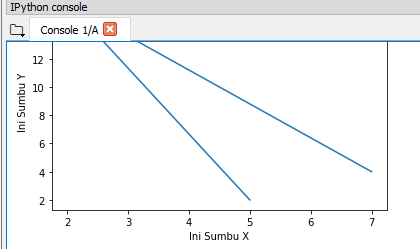
\includegraphics[width=9cm]{figures/6/Teori/1174096/1.png}
	\caption{Hasil membuat sumbu x dan y}
	\centering
\end{figure}

\subsection{Jelaskan bagaimana perbedaan fungsi dan cara pakai untuk berbagai jenis(bar,histogram,scatter,line dll) jenis plot di matplotlib}
Perbedaan fungsi dapat dilihat sebagai berikut :
\begin{itemize}
    \item Graph\linebreak
    Fungsi graph digunakan untuk membuat visualisasi berupa grafik.
    cara pakainya adalah sebagai berikut :
    \lstinputlisting[caption = fungsi untuk membuat graph., firstline=10, lastline=18]{src/6/Teori/1174096/1174096.py}
    hasilnya adalah sebagai berikut:
    \begin{figure}[H]
        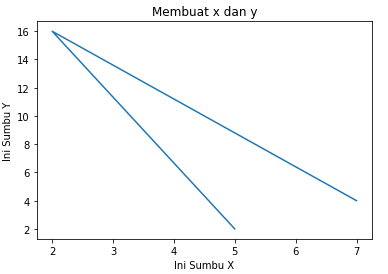
\includegraphics[width=9cm]{figures/6/Teori/1174096/3graph.png}
        \caption{Hasil graph}
        \centering
    \end{figure}

    \item Bar\linebreak 
    Fungsi Bar digunakan untuk membuat visualisasi berupa diagram batang yang berhimpit.
    Cara Pakainya adalah sebagai berikut :
    \lstinputlisting[caption = fungsi untuk membuat bar., firstline=22, lastline=32]{src/6/Teori/1174096/1174096.py}
    hasilnya adalah sebagai berikut:
    \begin{figure}[H]
        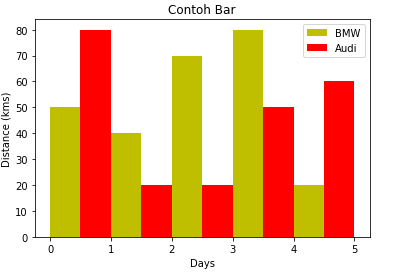
\includegraphics[width=9cm]{figures/6/Teori/1174096/3bar.png}
        \caption{Hasil bar}
        \centering
    \end{figure}

    \item Histogram\linebreak
    Fungsi Histogram digunakan untuk membuat visualisasi berupa diagram batang yang tidak berhimpit.
    Cara Pakainya adalah sebagai berikut :
    \lstinputlisting[caption = fungsi untuk membuat histogram., firstline=35, lastline=42]{src/6/Teori/1174096/1174096.py}
    hasilnya adalah sebagai berikut:
    \begin{figure}[H]
        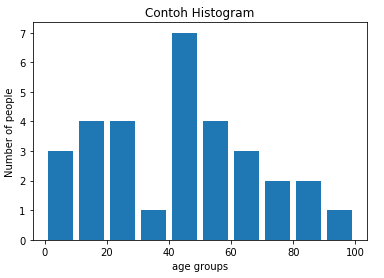
\includegraphics[width=9cm]{figures/6/Teori/1174096/3histogram.png}
        \caption{Hasil histogram}
        \centering
    \end{figure}

    \item Scatter\linebreak
    Fungsi Scatter digunakan untuk membuat visualisasi berupa titik titik.
    Cara Pakainya adalah sebagai berikut :
    \lstinputlisting[caption = fungsi untuk membuat scatter., firstline=45, lastline=58]{src/6/Teori/1174096/1174096.py}
    hasilnya adalah sebagai berikut:
    \begin{figure}[H]
        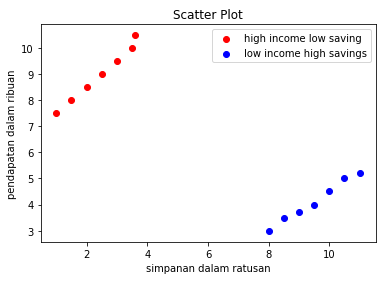
\includegraphics[width=9cm]{figures/6/Teori/1174096/3scatter.png}
        \caption{Hasil scatter}
        \centering
    \end{figure}

    \item Area plot\linebreak
    Fungsi Area plot digunakan untuk membuat visualisasi berupa area.
    Cara Pakainya adalah sebagai berikut :
    \lstinputlisting[caption = fungsi untuk membuat area plot., firstline=61, lastline=80]{src/6/Teori/1174096/1174096.py}
    hasilnya adalah sebagai berikut:
    \begin{figure}[H]
        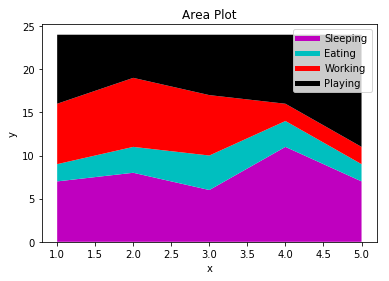
\includegraphics[width=9cm]{figures/6/Teori/1174096/3areaplot.png}
        \caption{Hasil area plot}
        \centering
    \end{figure}

    \item Pie\linebreak
    Fungsi Pie digunakan untuk membuat visualisasi berupa diagram lingkaran.
    Cara Pakainya adalah sebagai berikut :
    \lstinputlisting[caption = fungsi untuk membuat pie., firstline=83, lastline=104]{src/6/Teori/1174096/1174096.py}
    hasilnya adalah sebagai berikut:
    \begin{figure}[H]
        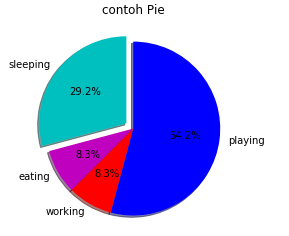
\includegraphics[width=9cm]{figures/6/Teori/1174096/3pie.png}
        \caption{Hasil pie}
        \centering
    \end{figure}
    
\end{itemize}

\subsection{Jelaskan bagaimana cara menggunakan legend dan label serta kaitannya dengan fungsi tersebut}
Fungsi legend digunakan untuk menjelaskan makna dari objek berupa titik atau garis di dalam diagram.
cara menggunakan legend adalah 
\lstinputlisting[caption = fungsi untuk membuat legend., firstline=24, lastline=28]{src/6/Teori/1174096/1174096.py}
contoh legend :
\begin{figure}[H]
    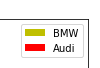
\includegraphics[width=9cm]{figures/6/Teori/1174096/4legend.png}
    \caption{contoh legend}
    \centering
\end{figure}

\subsection{Jelaskan apa fungsi dari subplot di matplotlib, dan bagaimana cara kerja dari fungsi subplot, sertakan ilustrasi dan gambar sendiri dan apa parameternya jika ingin menggambar plot dengan 9 subplot di dalamnya}
Subplot berfungsi untuk menggabungkan beberapa plot kedalam satu figure
cara kerjanya adalah sebagai berikut
\lstinputlisting[caption = cara kerja subplot., firstline=108, lastline=134]{src/6/Teori/1174096/1174096.py}
Parameter yang digunakan ketika ingin membuat 9 subplot terdiri dari (331) sampai (339). karena posisi subplot dilihat dengan melihat tinggi,lebar,urutan
hasil dari subplot adalah
\begin{figure}[H]
    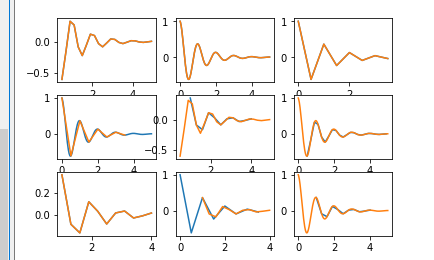
\includegraphics[width=9cm]{figures/6/Teori/1174096/5subplot.png}
    \caption{hasil subplot}
    \centering
\end{figure}

\subsection{Sebutkan semua parameter color yang bisa digunakan}
Parameter color yang bisa digunakan antara lain RGB dan CMYK
\begin{itemize}
    \item C (Cyan) adalah biru muda
    \item M (Magenta) adalah merah muda
    \item Y (Yellow) adalah kuning
    \item K (Key) adalah hitam
    \item R (Red) adalah merah
    \item G (Green) adalah Hijau
    \item B (Blue) adalah Biru
    
\end{itemize}

\subsection{Jelaskan bagaimana cara kerja dari fungsi hist, sertakan ilustrasi dan gambar sendiri}
cara kerja dari fungsi histogram adalah sebagai berikut :
\lstinputlisting[caption = cara kerja histogram., firstline=137, lastline=144]{src/6/Teori/1174096/1174096.py}
hasilnya adalah
\begin{figure}[H]
    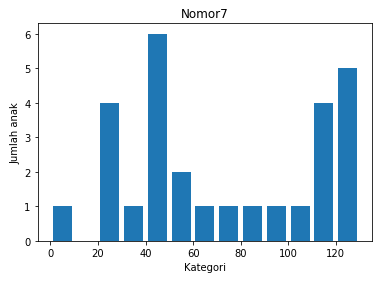
\includegraphics[width=9cm]{figures/6/Teori/1174096/7his.png}
    \caption{histogram}
    \centering
\end{figure}

\subsection{Jelaskan lebih mendalam tentang parameter dari fungsi pie diantaranya labels, colors, startangle, shadow, explode, autopct}
\begin{itemize}
    \item Labels = berfungsi untuk menampilkan tulisan pada diagram pie
    \item Colors = berfungsi untuk menentukan warna pada tiap bagian pada diagram pie
    \item Startangle = berfungsi untuk menentukan sudut pertama pada diagram pie
    \item Shadow = berfungsi untuk menampilkan efek timbul pada diagram pie
    \item Explode = berfungsi untuk menunjukkan jarak pisah dari diagram pie.
    \item Autopct = berfungsi umtuk menampilkan jumlah angka dibelakang koma pada bilangan pecahan
\end{itemize}

\subsection{Pengecekan Plagiarisme Teori}
\begin{figure}[H]
	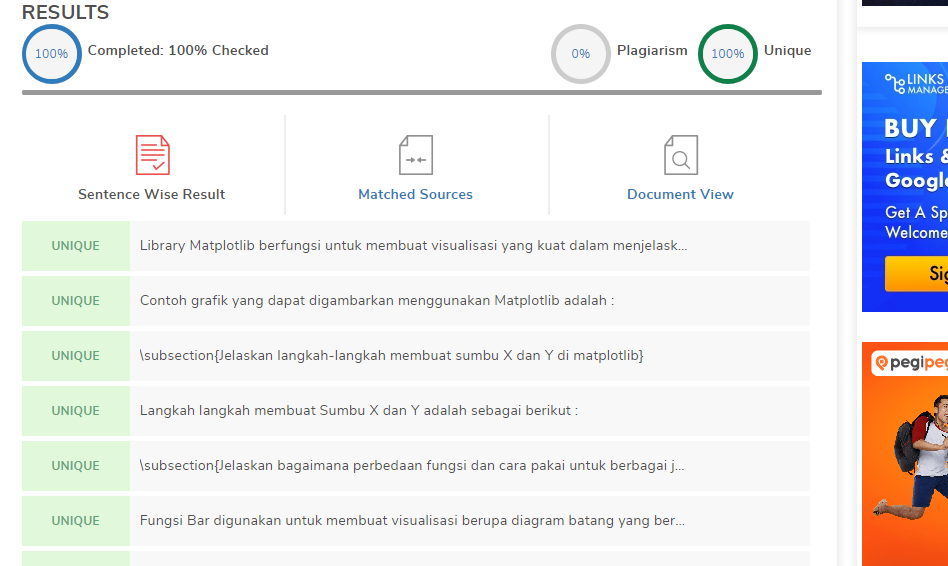
\includegraphics[width=9cm]{figures/6/Teori/1174096/Plagiat.png}
	\centering
\end{figure}

\section{Muhammad Dzihan Al-Banna}
\subsection{Soal 1}
Libarary matplotlib berfungsi untuk menampilkan data grafik yang mudah dibuat dan ditampilkan dengan cara sederhana saja di python yaitu hanya dengan mendefinisikan tabel x dan y kemudian mengisi variabelnya dengan data. Matplotlib sangat berguna untuk data science.
\subsection{Soal 2}
Membuat sumbu x dan y di matplotlib cukup mudah yaitu hanya dengan mengimport matplotlib terlebih dahulu, mendefinisikan fungsi plot dan membuat variable plot dan isi variable x dan y tersebut dengan data. Variable yang diisi pertama adalah sumbu x dan yang kedua adalah sumbu y.

\lstinputlisting[firstline=13, lastline=19]{src/6/Teori/1174095/T1174095_plt.py}
\subsection{Soal 3}
\begin{itemize}
\item Pada penggunaan bar di awal pembuatan fungsi ditambahkan plt.bar  yang pertama kemudian isi datanya, begitu juga yang kedua melakukan hal yang sama.
\lstinputlisting[firstline=22, lastline=32]{src/6/Teori/1174095/T1174095_plt.py}
\item dalam penggunaan histogram juga dilakukan coding seperti diatas pada bar tetapi menggunakan plt.hist
\item jika mau menggunakan fungsi scatter maka diganti dengan plt.scatter, jika menggunakan scatter maka grafiknya akan ditandai dengan titik.
\lstinputlisting[firstline=35, lastline=48]{src/6/Teori/1174095/T1174095_plt.py}
\end{itemize}
\subsection{Soal 4}
Membuat legend pertama-tama gunakan dulu style.use('ggplot') setelah itu buat plt.xlabel dan plt.ylabel sebagai penanda bahwa itu sumbu x dan y. setelah itu tambahkan plt.legend.
\lstinputlisting[firstline=51, lastline=66]{src/6/Teori/1174095/T1174095_plt.py}
\subsection{Soal 5}
\begin{figure}[h]
\centering
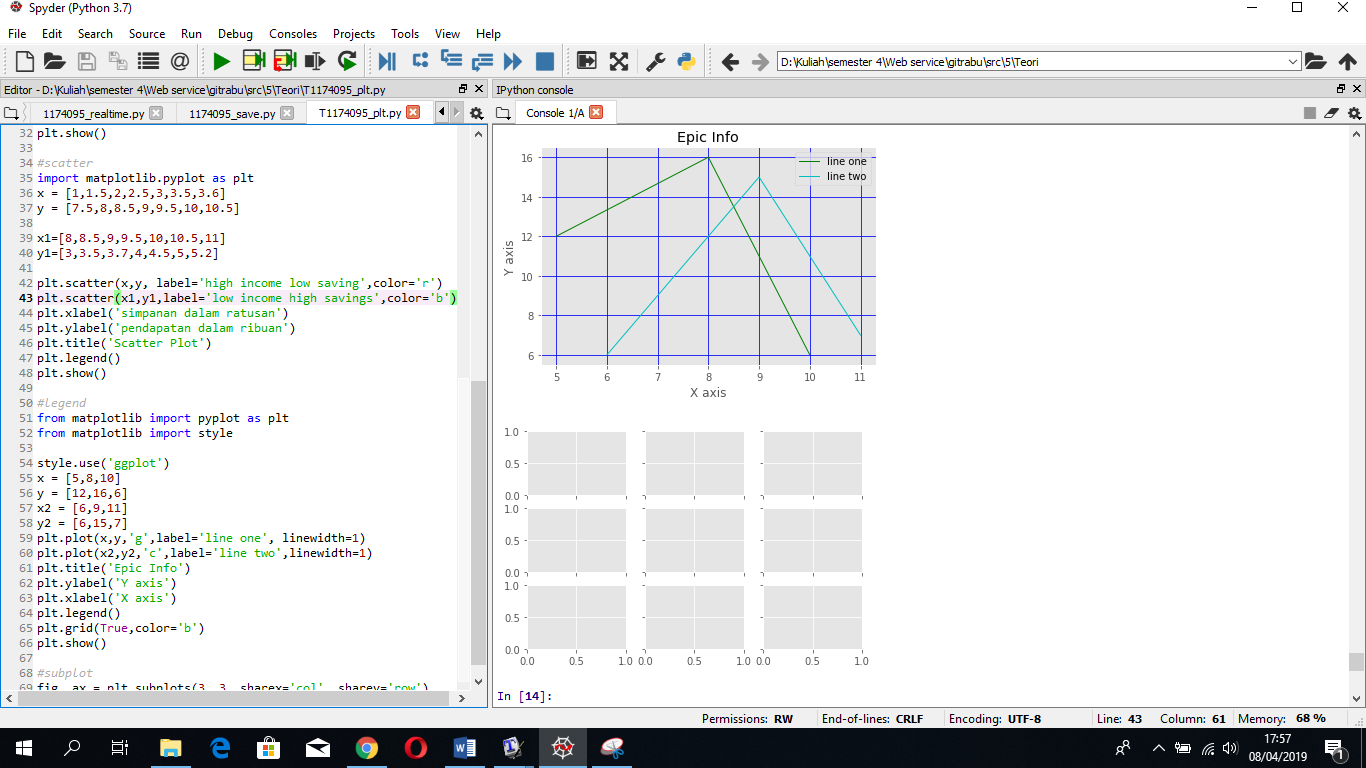
\includegraphics[width=20cm]{figures/6/Teori/1174095/ssub.png}
\caption{Sub Plot}
\label{Dzihan}
\end{figure}
sublot berfungsi untuk menampilkan banyak plot dalam satu grafik.
\begin{itemize}
\item buat fungsi subplot
\item isi parameternya
\item definisikan colomn dan rownya.
\item atur range yang ingin ditampilkan
\item Jika ingin membuat 9 sublot maka atur rangenya menjadi 3,3 agar rownya terisi 3 dan coloumnnya 3.
\end{itemize}
\subsection{Soal 6}
Parameter color yang bisa digunakan dalam library maplotlib adalah RGB dan CMYK.
\subsection{Soal 7}
Cara untuk menampilkan hist adalah dengan menggunakan plt.hist. caranya adalah sebagai berikut :
\lstinputlisting[firstline=72, lastline=79]{src/6/Teori/1174095/T1174095_plt.py}
\subsection{Soal 8}
\begin{enumerate}
\item label digunakan untuk menandai bagian tertentu seperti sumbu x atau sumbu y
\item colors digunakan untuk memberikan warna di bagian table pada data grafik
\item startangle digunakan untuk memutar balikan table dengan arah kebalikannya.
\item shadow digunakan untuk memberikan bayangan pada data agar terlihat seperti 3D.
\item explode digunakan untuk menonjolkan data dari grafik tertentu agar terlihat lebih mencolok.
\item autocpt digunakan untuk memberi persen pada bagian paychart yang dibuat.
\end{enumerate}

Kalau mau dibikin paragrap \textbf{cukup enter aja}, tidak usah pakai \verb|par| dsb

%\subsection{Soal 2}
%Isi jawaban soal ke-2

%\subsection{Soal 3}
%Isi jawaban soal ke-3

\section{Harun Ar-Rasyid}
\subsection{Soal 1}
Isi jawaban soal ke-1

Kalau mau dibikin paragrap \textbf{cukup enter aja}, tidak usah pakai \verb|par| dsb

%\subsection{Soal 2}
%Isi jawaban soal ke-2

%\subsection{Soal 3}
%Isi jawaban soal ke-3

\section{Sri Rahayu}
\subsection{Soal 1}
Isi jawaban soal ke-1

Kalau mau dibikin paragrap \textbf{cukup enter aja}, tidak usah pakai \verb|par| dsb

%\subsection{Soal 2}
%Isi jawaban soal ke-2

%\subsection{Soal 3}
%Isi jawaban soal ke-3

\section{Doli Jonviter}
\subsection{Soal 1}
Isi jawaban soal ke-1

Kalau mau dibikin paragrap \textbf{cukup enter aja}, tidak usah pakai \verb|par| dsb

%\subsection{Soal 2}
%Isi jawaban soal ke-2

%\subsection{Soal 3}
%Isi jawaban soal ke-3

\section{Rahmatul Ridha}
\subsection{Soal 1}
Isi jawaban soal ke-1

Kalau mau dibikin paragrap \textbf{cukup enter aja}, tidak usah pakai \verb|par| dsb

%\subsection{Soal 2}
%Isi jawaban soal ke-2

%\subsection{Soal 3}
%Isi jawaban soal ke-3

\section{Tomy Prawoto}
\subsection{Soal 1}
Isi jawaban soal ke-1

Kalau mau dibikin paragrap \textbf{cukup enter aja}, tidak usah pakai \verb|par| dsb

%\subsection{Soal 2}
%Isi jawaban soal ke-2

%\subsection{Soal 3}
%Isi jawaban soal ke-3
